\chapter{System Analysis and Design}
This chapter describes the study, analysis and design of the system. It highlights the identified requirements and architectural design of the system.

\section{Overview of the system}
The system designed in this project is aimed at having students’ transcripts stored and shared on a blockchain network. The storage of transcripts on a blockchain network ensures more security in addition to their storage as hard copy documents.
To emphasize security, the transcripts are first hashed into data of fixed size and then stored on a blockchain. The system uses IPFS (InterPlanetary File System)\cite{art16} to produce a hash code for a transcript. The resultant hash code is then stored on the Ethereum blockchain.\\
In order to simulate the blockchain locally, this system uses Ganache\cite{art17} which runs a local instance of the Ethereum blockchain on a user computer. To gain access to the network, the user needs a browser extension known as MetaMask. MetaMask is a bridge that allows users to visit the distributed web through their browsers. It allows one to run Ethereum dApps\cite{art18} right in one's browser. Addition of each transcript to the blockchain costs a certain amount of ether\cite{art19}, the currency for the Ethereum blockchain.
\begin{figure}[H]
\centering
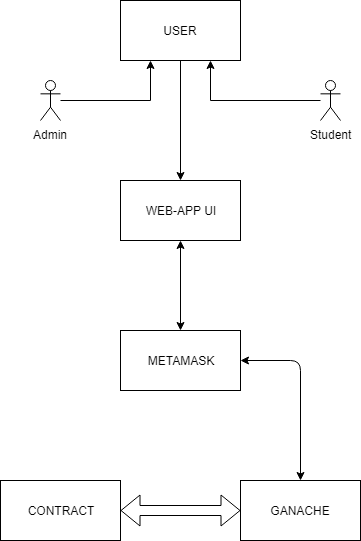
\includegraphics[scale=0.8]{images/simple_system.png}
\caption{Simple system Architecture}
\end{figure}
\section{System Analysis}
\subsection{Data Analysis}
From the data retrieved during the research process, we found that the present system handling students’ records is prone to a number of errors and weaknesses.\\\\
The current system handling students’ results at Makerere University does not have a limit to the number of times a student can do a course as opposed to the actual policy by the University where a student is meant to sit for exams in a course not more than three times.\\\\
Another discovery from the data received was that the present-day system handling students’ results at Makerere University can accept an input of a percentage figure greater than 100\%.\\\\
Another important note is that currently, students' transcripts exist only in hard copy and can only be picked and verified at the University.

\subsection{System Requirements}
The system uses IPFS and the Ethereum blockchain as its main foundation. MetaMask is a browser extension required for user access to the Ethereum blockchain  via a browser e.g. Google Chrome, Mozilla Firefox among others. Below are the user requirements, functional and non-functional requirements.

\subsubsection{User Requirements}
\begin{enumerate}
\item[U.1] Allow an administrative assistant enter students’ results.
\item[U.2] Allow students to access their results without being able to change them.
\item[U.3] Provide for students to easily share their results information with employers.
\item[U.4] Allow employers to easily verify students' results.
\end{enumerate}

\subsubsection{Functional Requirements}
\begin{enumerate}
\item[F.1] Ensure user authentication through login.
\item[F.2] Reject addition of inaccurate results.
\item[F.3] Ensure that the students’ results are not altered.
\item[F.4] Ensure students' transcript can be saved locally.
\item[F.5] Uploading transcript to IPFS.
\item[F.6] Saving IPFS hash to the blockchain.
\end{enumerate}

\subsubsection{Non Functional Requirements}
\begin{enumerate}
\item[N.1] The system must verify any addition to the blockchain.
\item[N.2] The system must notify the system administrator incase of any unauthorized / filed transactions.
\end{enumerate}

Below is a use case diagram depicting the interactions among the system's elements.
\subsubsection{Use Case Diagram}
\begin{figure}[H]
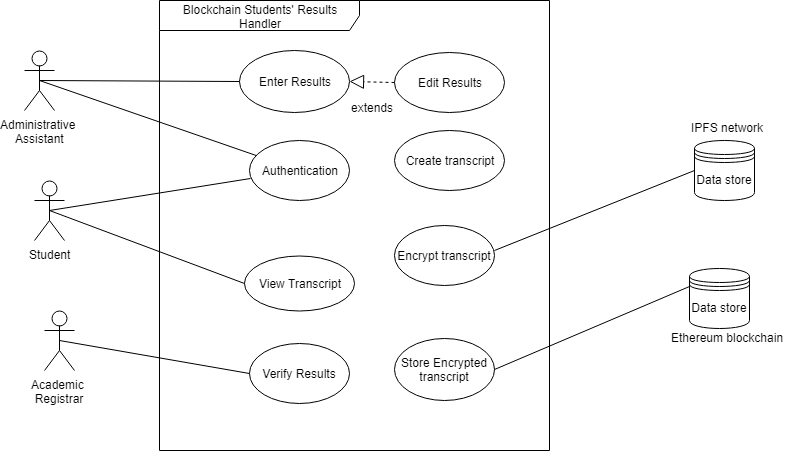
\includegraphics[scale=0.5]{images/UseCaseDiagram.png}
\caption{Use Case diagram}
\end{figure}

\section{System Design}
The system is dependant on two technologies i.e IPFS and Ethereum. This section includes an overview of how each of these technologies work.
\begin{itemize}
\item\textbf{IPFS}\\
IPFS is an open-source, peer-to-peer distributed hypermedia protocol that aims to function as a ubiquitous file system for all computing devices. It is a complex and highly ambitious project with some serious and profound implications on the future development and structure of the Internet as we know it.\\
\begin{figure}[H]
  \caption{IPFS decentralized architecture.}
  \centering
  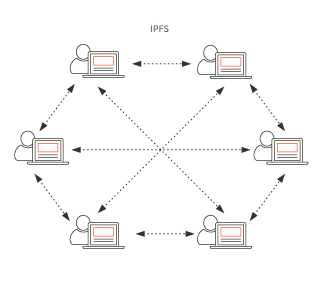
\includegraphics[width=0.9\textwidth]{images/IPFS.png}
\end{figure}
The links between the nodes in IPFS take the form of cryptographic hashes, and this is possible because of its Merkle DAG\cite{art20} (Directed Acyclic Graphs) data architecture. Each file and all blocks within it are given a unique identifier, which is a cryptographic hash. Duplicates are removed across the network and version history is tracked for every file.\\\\
\item\textbf{Ethereum blockchain}\\
Ethereum's architecture allows for an application to sign transactions offline and relay them to a public node. In this project, since we are running a local instance of the blockchain using Ganache, we have set up a web3 provider engine in our configuraion to transparently sign transactions offline, using Metamask, and send them to an IPFS node.
\begin{figure}[H]
  \caption{Ethereum blockchain architecture with offline Signing and public nodes.}
  \centering
  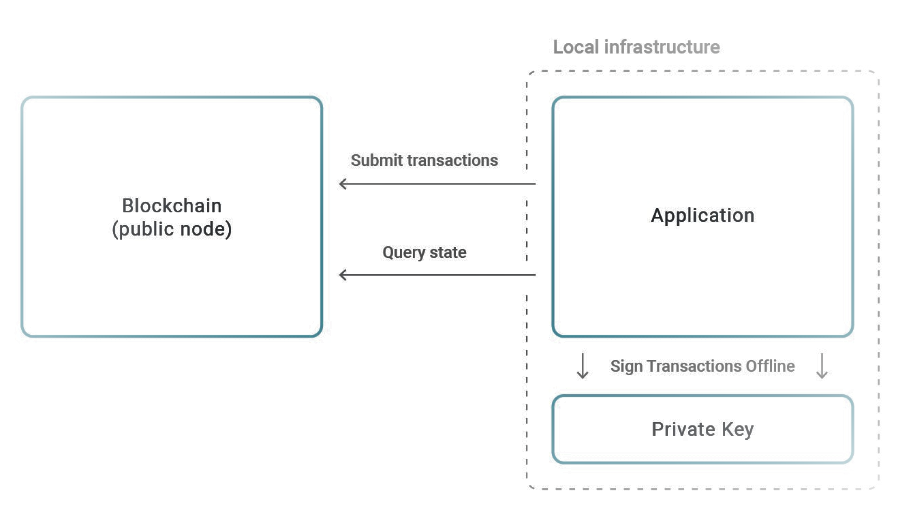
\includegraphics[width=0.9\textwidth]{images/OfflineBlockchainarch.png}
\end{figure}
\end{itemize}

\subsection{System Architecture}
The structure of the system is composed of the following major components:
\begin{itemize}
\item A blockchain network built on the Ethereum platform and a local implementation of it running in Ganache.
\item The IPFS distributed network for storage and peer-to-peer sharing of records.
\item A students' results system that combines:
\begin{enumerate}
\item Creation and Manipulation of results locally
\item Storage, Access and distribution of results remotely
\end{enumerate}
\item A storage server for student information and transcripts
\end{itemize}
Below is a class diagram describing the structure of the system.

\subsubsection{Class Diagram}
\begin{figure}[H]
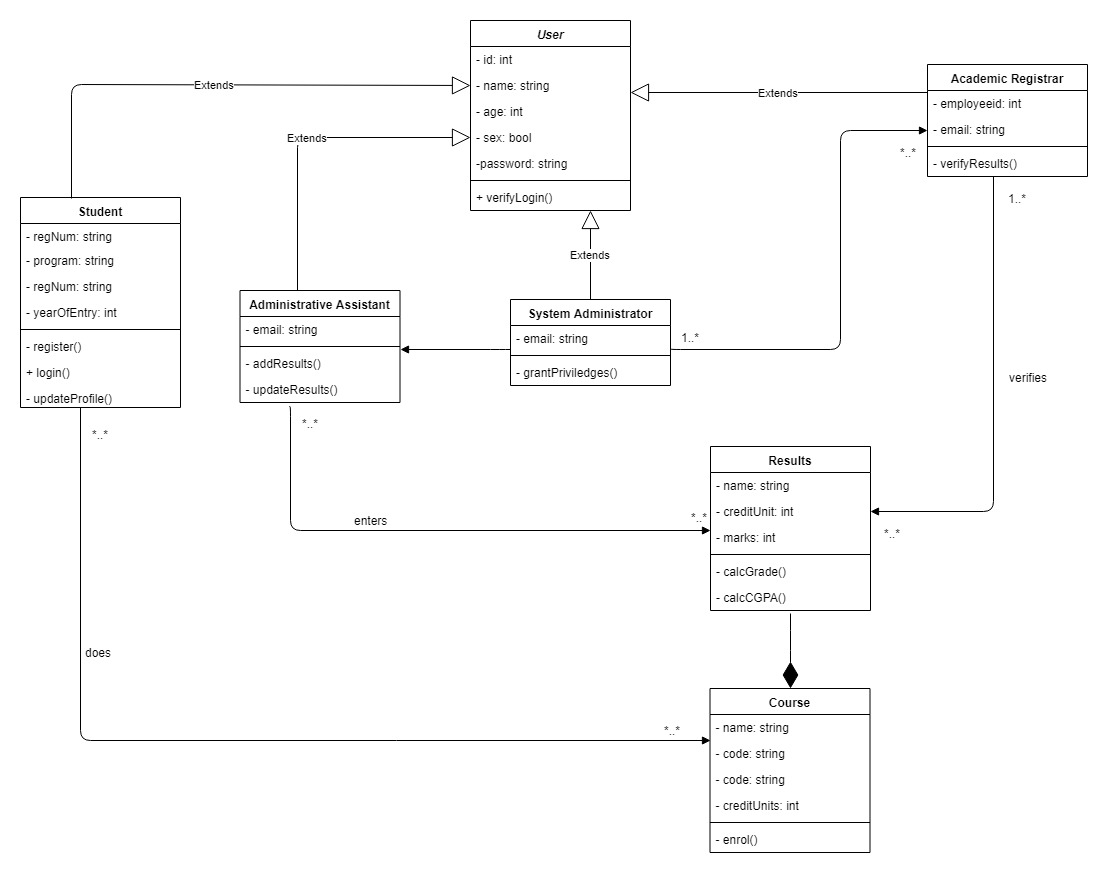
\includegraphics[scale=0.4]{images/class.jpg}
\caption{Class diagram}
\end{figure}

\subsection{Design Constraints}
The system for storing students' results on the blockchain is dependent on a number of factors, and these constrain its design in one way or another. Here below are some example constraints: 
\begin{itemize}
\item \textbf{\textit{Internet Connectivity}}\\
Since the system runs online, this thereby implies the need for users to have access to the internet.
\item \textbf{\textit{Browser Support}}\\
Any browser can be used to access the internet. However, accessing the Ethereum blockchain to use a dApp via a browser needs that particular browser to support the MetaMask extension. Currently, Metamask extensions are only available for Chrome, Firefox, Opera and Brave browsers. This constrains the system to these particular browsers, leaving out users that may not have the mentioned browsers.
\item \textbf{\textit{Payment for the blockchain (in Cryptocurrency)}}\\
Writing to the blockchain costs gas. Gas in the context of Ethereum is a unit and a measurement for the computing power that is needed to execute certain operations in the Ethereum Virtual Machine (EVM). Use of the system would require an Ethereum wallet\cite{art21}.
\item \textbf{\textit{The Ganache limitation}}\\
During simulation of the blockchain network locally and implementation of the system using Ganache, the developers were limited to only ten virtual accounts to simulate the entire network of actual accounts.
\end{itemize}
\textbf{Assumptions}\\
Some assumptions were made during the design and development of the system. They include the following:\\
\begin{itemize}
\item The end-user is willing to learn and adopt to the technology that may be new to him/her.
\item Users have a reliable connection to the internet.
\item Users are familiar with common internet browsers and file extensions for these browsers.
\item The system uses QR codes for purposes of verification. Therefore, it is assumed that users are familiar with QR codes and have access to a QR code scanner.
\item Scalability of the system will not negatively affect the application’s speed and reliability.
\end{itemize}

\subsection{Design Methodology}
We used the Agile software development (ASD) methodology. This methodology involves adaptive planning, evolutionary development, early delivery, and continual improvement. It also encourages rapid and flexible response to change. We focused on keeping code simple and testing often. This helped us to minimize risks such as bugs, cost overruns and the changing requirements.

\subsection{Graphical User Interface (GUI) Design}
This section provides the detailed design of the system and subsystem inputs and outputs relative to the user.

\subsubsection{Inputs}
\begin{itemize}
\item \textbf{\textit{User Credentials for Authentication:}} - Access to the Resuslts system requires User Authentication depending on whether a user is an Administrator or Student. 
\item \textbf{\textit{MetaMask Password:}} - In order for users to access the blockchain through their browser and via the Metamask, the extension requires a user password. Upon account creation on MetaMask, users are given a secret seed phrase. This seed phrase can be used for password recovery and for first time usage on a different device.
\item \textbf{\textit{Results:}} - When an administrative assistant logs into the system, he/she can enter the students’ results.
\end{itemize}

\subsubsection{Outputs}
\begin{itemize}
\item \textbf{\textit{Testimonial:}} - This is progressively updated and available on the Results system. Before the results are forwarded to the blockchain, a student can access the system and view his/her progressive results.
\item \textbf{\textit{Transcript:}} - Upon completion of study, a students can view their transcripts which can be downloaded as a pdf document for purposes of printing. This pdf is then digitized and encrypted before it is shared and stored on a global network. Students have access to their transcripts from anywhere and the will to share it with employers.
\end{itemize}

\subsection{External Interfaces}
\subsubsection{Hardware Interfaces}
The Results System needs access to a local server for storage of testimonials and transcripts locally. These could also be backed up on a cloud server, depending on the institution's particular system.\\\\
To access the functionality of this system, a user is required to have a computer with internet connection and a browser that supports the MetaMask extension. These browsers include Google chrome, Mozilla Firefox, among others) with the MetaMask browser extension installed. 

\subsubsection{Software Interfaces}
The functionalities of the external interfaces were developed using web-based scripting langauages like PHP, JavaScript and the smart contract for the Ethereum blockchain written in solidity.